\documentclass{beamer}
\usepackage{caption}
\usepackage{subfigure}
\usetheme[background=light]{metropolis}

\title{A Presentation of our Work}
\date{2016-08-18}
\author{The Swedish Interns}
\institute{Created for NVI Inc. at the Goddard Space Flight Centre}

\begin{document}
    \maketitle

%    \begin{frame}{Table of Contents}
%    \tableofcontents
%    \end{frame}

%%%%%%%%%%%%%%%%%%%%%%%%%%%%%%%%%%%%%%%%%%%%%%%%%%%%%%%%%%%%%%%%%%%%%%%%%%%%%%%

    \section{Weeks 1-2: Learning Fortran}

    \begin{frame}{Calculator}
        \begin{figure}[ht]
            \centering
            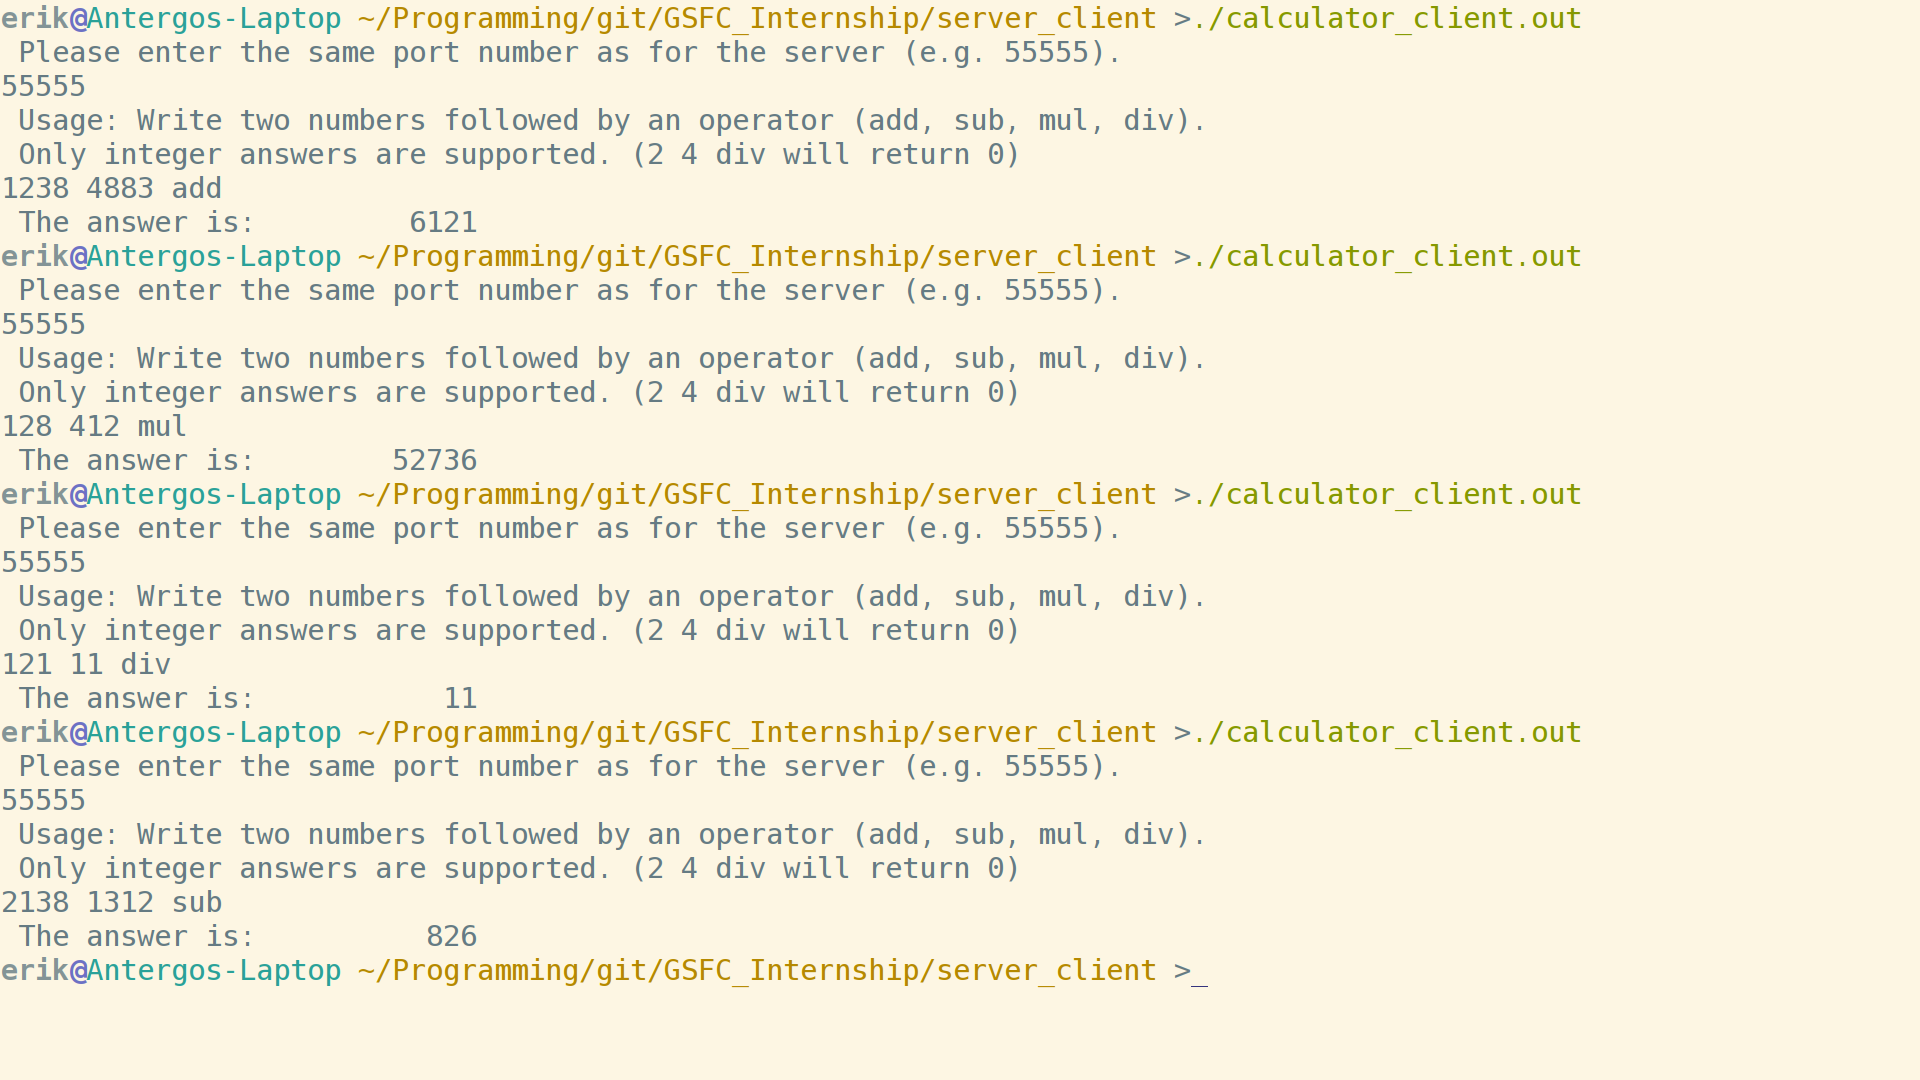
\includegraphics[width=1\columnwidth]{calculator}
            \caption{Example usage of the TCP calculator.}
        \end{figure}
    \end{frame}

%%%%%%%%%%%%%%%%%%%%%%%%%%%%%%%%%%%%%%%%%%%%%%%%%%%%%%%%%%%%%%%%%%%%%%%%%%%%%%%

    \section{Weeks 3-7: Our First Project}

    \begin{frame}
        Rewrite how globl/solve handles its passing of data to and from
        usrpartials and usrprogs.

        By minimizing disc I/O we want to increase the speed at which data is
        sent.
    \end{frame}

%%%%%%%%%%%%%%%%%%%%%%%%%%%%%%%%%%%%%%%%%%%%%%%%%%%%%%%%%%%%%%%%%%%%%%%%%%%%%%%
    \section{Week 3-4: Testing I/O performance}

    \begin{frame}{I/O Performance}
    \begin{itemize}[<+->]
        \item A couple of contenders:
            \begin{itemize}
                \item Read/Write with files
                \item Read/Write with pipes
                \item Sending/Receiving with TCP Sockets
                \item Sending/Receiving with OpenMPI
                \item Sending/Receiving with ZeroMQ (ØMQ)
            \end{itemize}
    \end{itemize}
    \end{frame}
%%
    \begin{frame}{Performance Test}
        \begin{enumerate}[<+->]
            \item The producer generates a list of length n and fills it with
                  integers.
            \item The producer writes the list to file (or sends it over the
                  designated transfer protocol).
            \item The consumer reads (or receives) the list.
            \item The consumer squares each int in the list and sends it back
                  to the producer.
            \item The producer reads (or receives) the modified list.
        \end{enumerate}
    \end{frame}

%%
    \begin{frame}{Result for I/O Performance}
    \begin{figure}[h!]
        \centering
        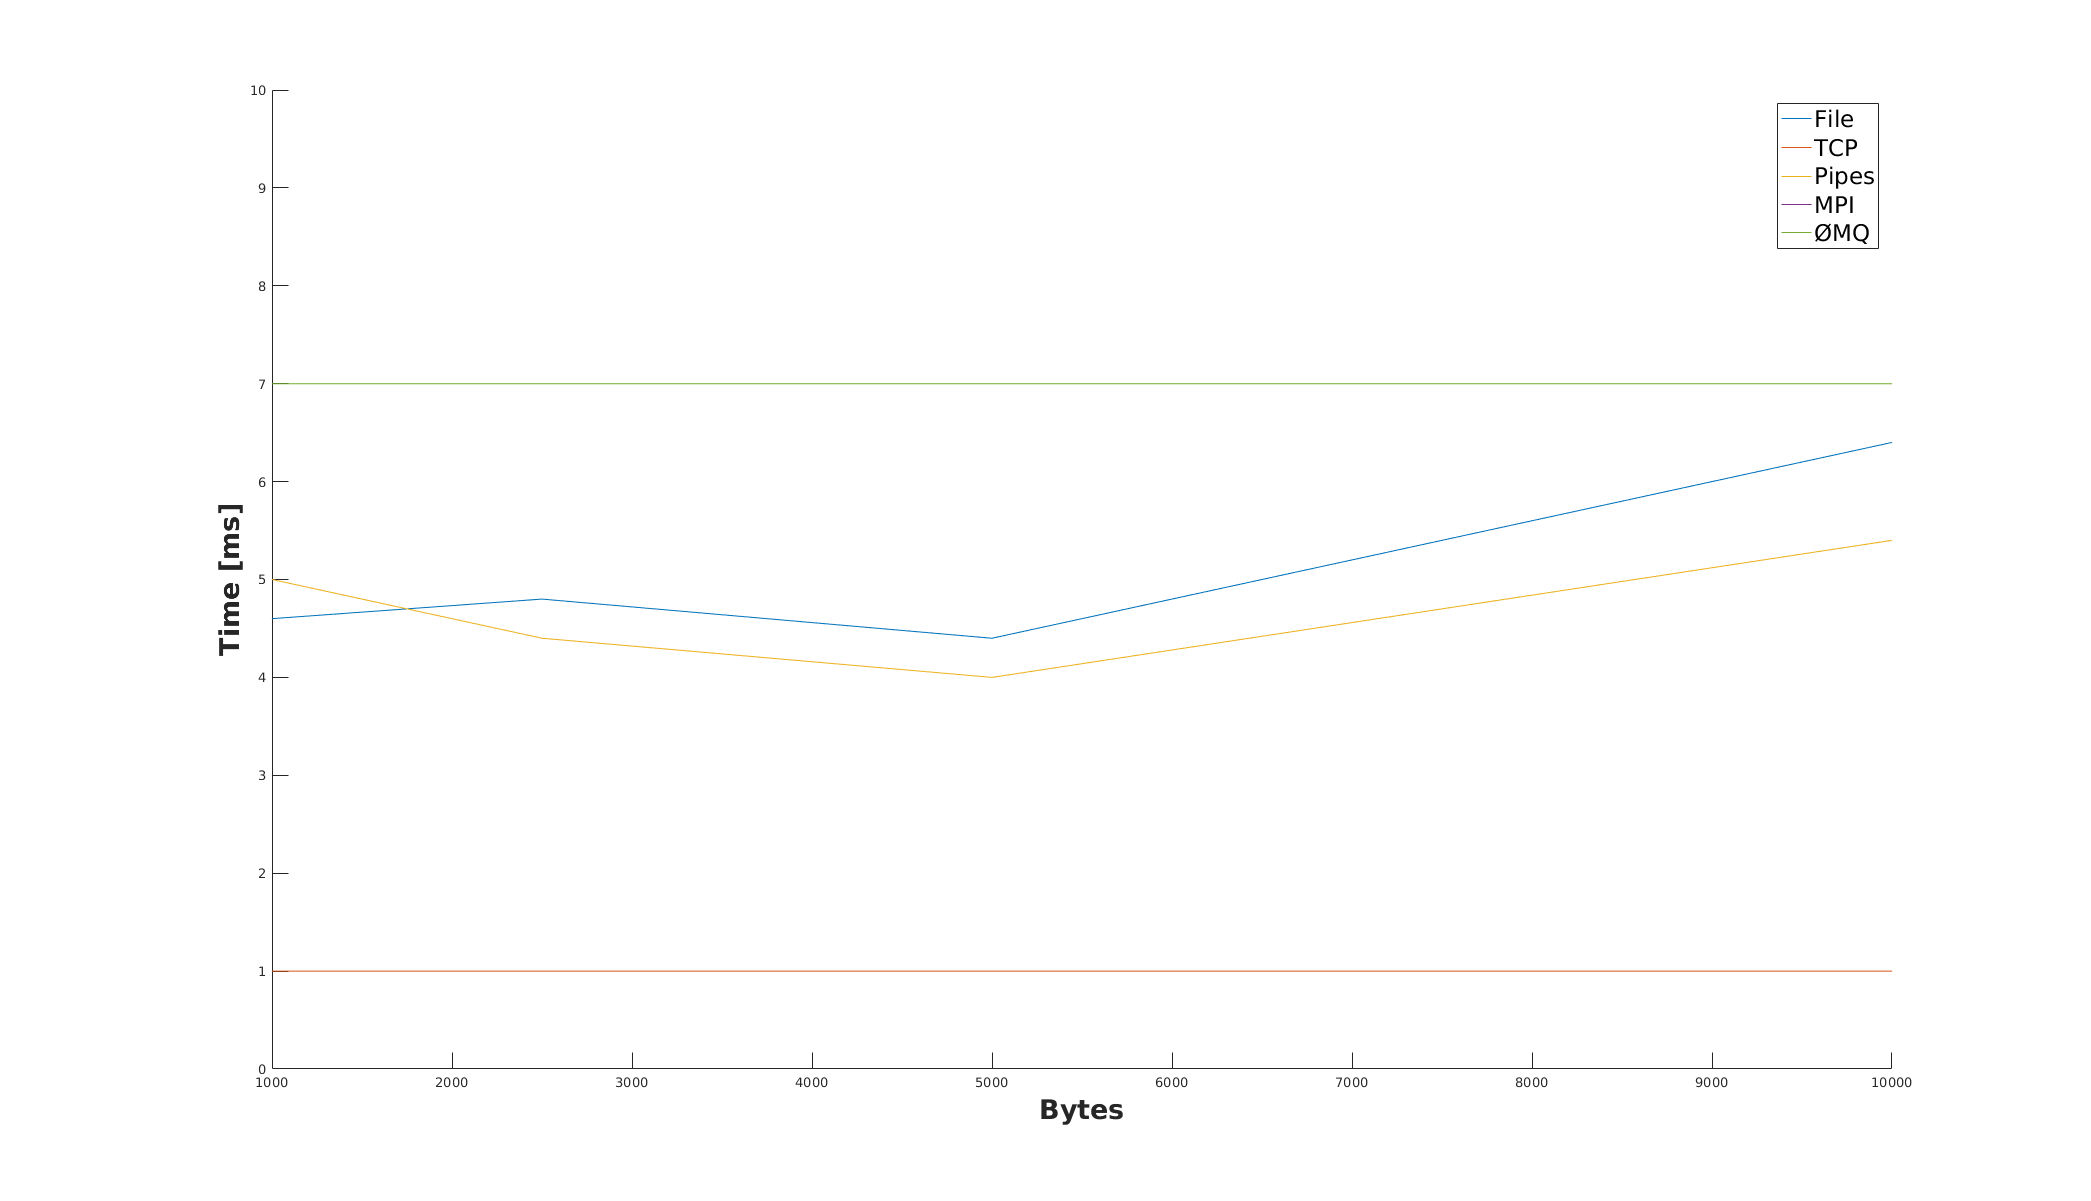
\includegraphics[width=1\columnwidth]{singlerun-nf}
    \end{figure}
    \end{frame}
%%
    \begin{frame}{Result for I/O Performance}
    \begin{figure}[h!]
        \centering
        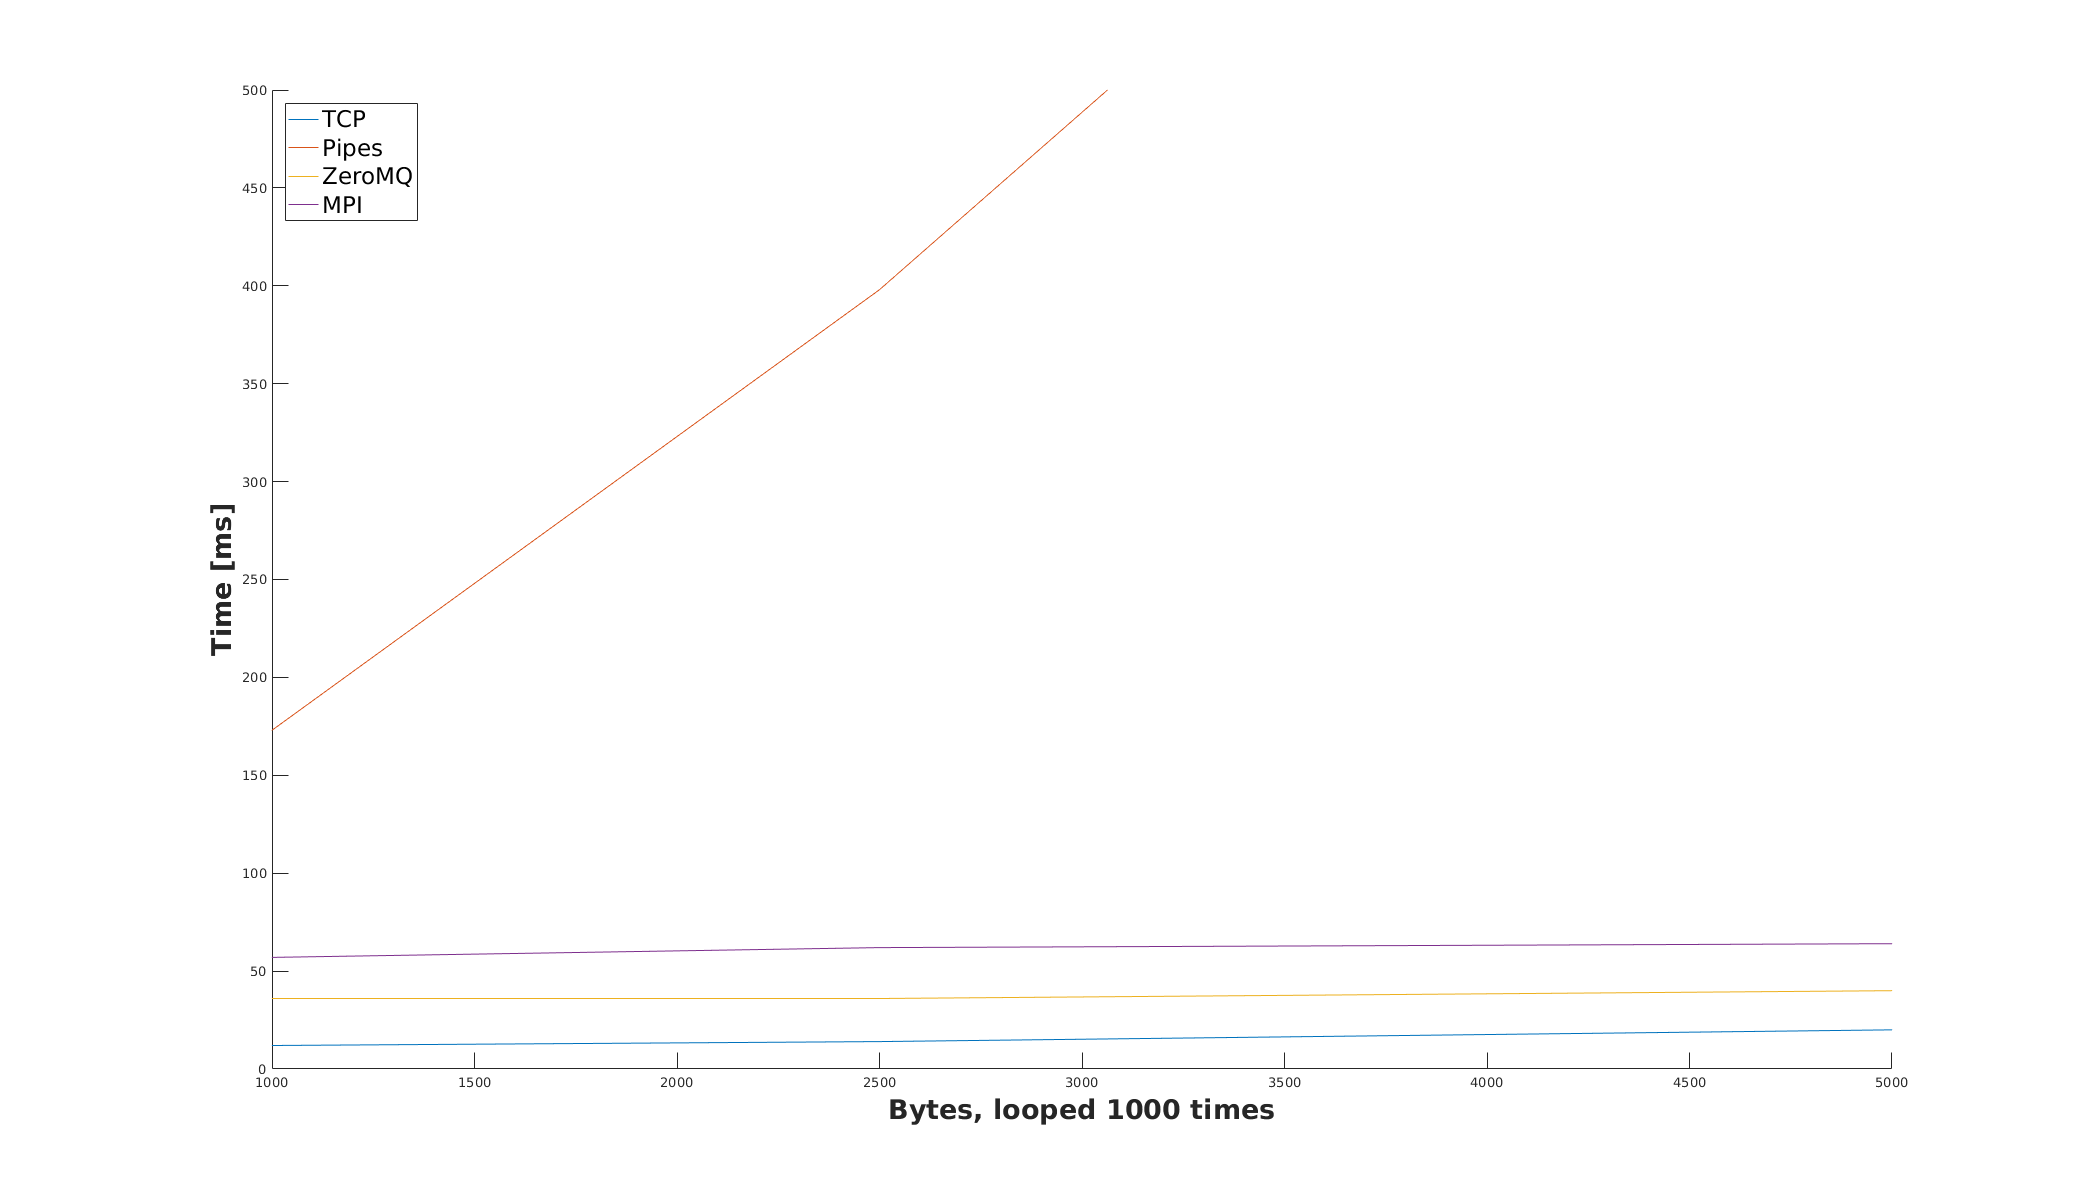
\includegraphics[width=1\columnwidth]{thousandrun-nf}
    \end{figure}
    \end{frame}
%%
    \begin{frame}{Result for I/O Performance}
    \begin{itemize}[<+->]
        \item TCP was the fastest, but the most difficult to implement.
        \item Since we assumed a lot of data would be passed we opted for ØMQ
              due to its presumptive ease of use and performance.
    \end{itemize}
    \end{frame}

%%%%%%%%%%%%%%%%%%%%%%%%%%%%%%%%%%%%%%%%%%%%%%%%%%%%%%%%%%%%%%%%%%%%%%%%%%%%%%%

    \section{Weeks 5-7: Implementation}

    \begin{frame}{Implementation}
    \begin{itemize}[<+->]
        \item Installation of Software on \bf{bootes}
        \item Porting our code to ifort
        \item A lot of coding.
    \end{itemize}
    \end{frame}

%%%%%%%%%%%%%%%%%%%%%%%%%%%%%%%%%%%%%%%%%%%%%%%%%%%%%%%%%%%%%%%%%%%%%%%%%%%%%%%

    \section{Results for Project One}

    \begin{frame}{Results for Project One}
    \begin{figure}[h!]
        \centering
        \includegraphics[width=1\columnwidth]{p1res1}
    \end{figure}
    \end{frame}

    \begin{frame}{Results for Project One}
    \begin{figure}[h!]
        \centering
        \includegraphics[width=1\columnwidth]{p1res2}
    \end{figure}
    \end{frame}

    \begin{frame}{Results for Project One}
        \centering{Why?}
    \end{frame}

    \begin{frame}{Results for Project One}
        \begin{itemize}[<+->]
            \item Turns out we are competing 
        \end{itemize}

    \end{frame}

\end{document}

